\documentclass[11pt]{article}
\usepackage{amsmath,amssymb,amsthm}
\usepackage{graphicx}
\usepackage[margin=1in]{geometry}
\usepackage{fancyhdr}
\usepackage{graphicx}
\usepackage{subcaption}
\setlength{\parindent}{0pt}
\setlength{\parskip}{5pt plus 1pt}
\setlength{\headheight}{13.6pt}
\newcommand\question[2]{\vspace{.25in}\hrule\textbf{#1: #2}\vspace{.5em}\hrule\vspace{.10in}}
\renewcommand\part[1]{\vspace{.10in}\textbf{#1}}
\pagestyle{fancyplain}
\lhead{\textbf{\NAME\ (\ANDREWID)}}
\chead{\textbf{HW\HWNUM}}
\rhead{\today}

\begin{document}\raggedright
	\newcommand\NAME{Muhammed Burak Bugrul}
	\newcommand\ANDREWID{150140015}
	\newcommand\HWNUM{1}
	\question{Q1}{PEAS}
	PEAS stands for (P)erformance Measure, (E)nvironment, (A)ctuators, (S)ensors. PEAS analysis for a domestic service robot is:
	
	\textbf{Observable:} Partially \\
	\textbf{Determinism:} Stochastic \\
	\textbf{Episodic:} Sequential \\
	\textbf{Static:} Dynamic \\
	\textbf{Discrete:} Continuous \\
	\textbf{Agents:} Multi \\ \ \\
	
	I would choose the \textbf{'Learning Agent Architecture'} for this agent because it should measure the performance and outcomes of its own actions and improve/adjust its behaviours according to feedbacks.
	\question{Q2}{Heuristic}
	
	In this part, I will use the notation from our course slides:\\ \ \\
	
	$h(n)$ - heuristic cost of node $n$.\\
	$c(n, a, n')$ - real cost of action to advance from node $n$ to node $n'$\\
	$r(n)$ - real cost from node $n$ to a goal node.\\ \ \\
	
	For consistency:
	$$h(n) \leq c(n, a, n') + h(n')$$
	condition should be satisfied. In the goal node, $h(goal)$ and $r(goal)$ is 0. For any other node $n$, there should be at least one node $n'$ that satisfies:
	$$r(n') = r(n) - 1$$
	
	In admissibility $h(n') \leq r(n')$ condition should be true, so we can change the first condition to:
	$$h(n) \leq c(n, a, n') + r(n')$$
	as we know $c(n, a, n') + r(n') = r(n)$, it takes us to $h(n) \leq r(n)$.
	
	For an example of a heuristic that is admissible but inconsistent, let's examine the graph given below:
	
	\begin{figure}[h!]
		\centering
		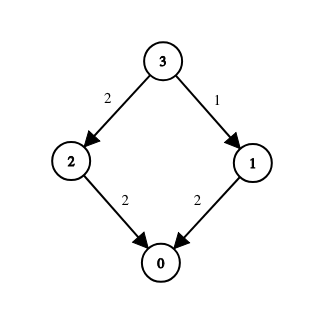
\includegraphics[width=0.18\textwidth]{images/graph.png}
		\caption{Graph}
		\label{fig:Graph}
	\end{figure}

	In this graph, heuristic costs are given in nodes and action costs are given on edges. The node that has 0 heuristic cost is the goal node and the node has 3 heuristic cost is the initial node. $h(n) \leq r(n)$ is satisfied for all nodes. But heuristic cost of 3 is bigger than heuristic cost of 1 + actual cost of 1(edge between them)
	
	
	\question{Q3}{Peg Problem}
	In this part, we are wanted to implement and analyze BFS, DFS and A* algorithms on given peg problem.\\
	\part{Problem Formulization} \\ \ \\
	\textbf{State:} A 7x7 matrice of 1s and 0s. 1s represent holes with pegs in them and 0's represent empty holes.\\
	\textbf{Action:} Making a peg jump orthogonally over an adjacent peg into an empty hole and then the jumped peg is removed. This action creates a new state.\\
	\textbf{Initial State:} State that given in the picture in the assignment pdf.\\
	\textbf{Goal State:} Any state that can make no valid action.\\
	\textbf{Path Cost:} Evey peg move counts with the same cost in this problem. So, path cost is the number of actions.\\
	
	\part{Algorithms} \\ \ \\
	
	You can compile the codes with the \texttt{'sh compile\_all.sh'} command.\\
	
	\part{BFS Algorithm} \\ \ \\
	
	You can run the algorithm with the \texttt{'./bfs'} command.\\
	
	BFS expands a lot of unnecessary node due to its Breadth first iteration but in this problem it is guaranteed for BFS to find an optimal solution. Because all actions costs are same. Here is the analysis of the BFS run:
	
	\begin{figure}[h!]
		\centering
		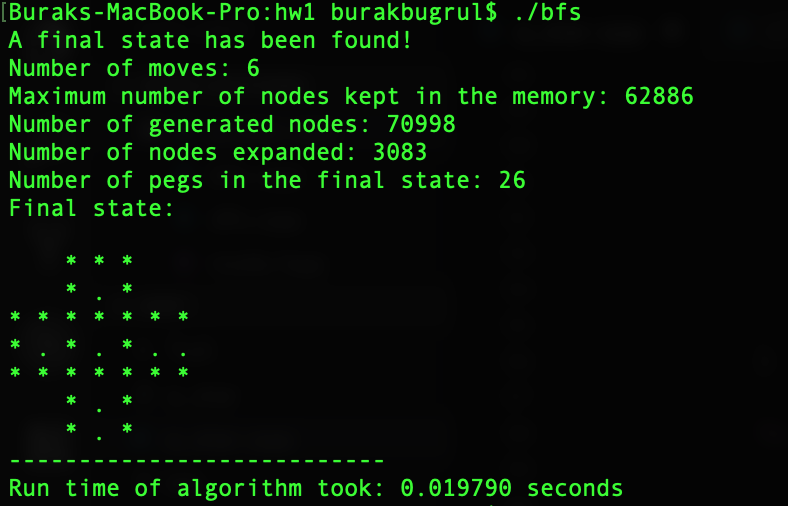
\includegraphics[width=0.5\textwidth]{images/bfs.png}
		\caption{BFS}
		\label{fig:BFS}
	\end{figure}

	\cleardoublepage

	\part{DFS Algorithm} \\ \ \\
	
	You can run the algorithm with the \texttt{'./dfs'} command.\\
	
	DFS expands always the first node it explores due to its depth first iteration. In this problem it is not guaranteed for DFS to find an optimal solution. Because it can explore a longer path to a close child. Here is the analysis of the DFS run:
	
	\begin{figure}[h!]
		\centering
		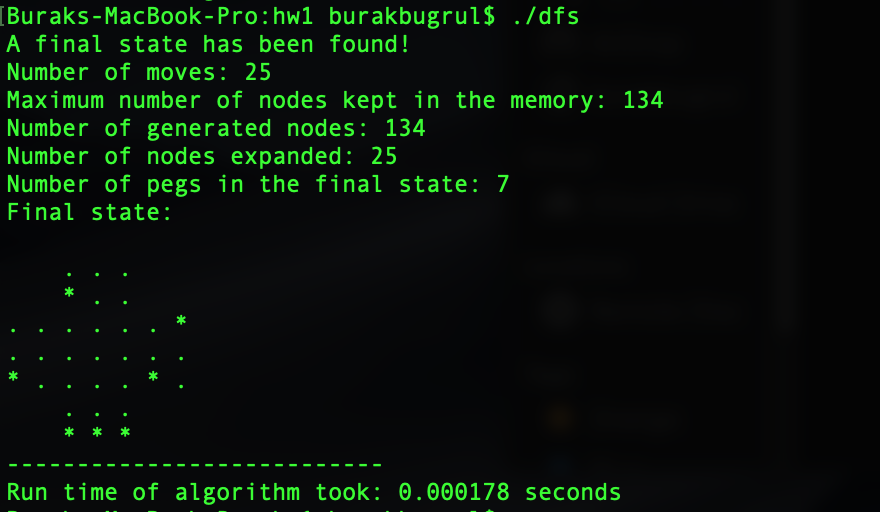
\includegraphics[width=0.5\textwidth]{images/dfs.png}
		\caption{A boat.}
		\label{fig:DFS}
	\end{figure}	

	\part{A* Algorithm} \\ \ \\
	
	You can run the algorithm with the \texttt{'./a\_star 1'} or \texttt{'./a\_star 2'} command.\\
	
	Independent from the problem, it is guaranteed for A* to find an optimal solution with an admissible and consistent heuristic function. In this problem, I analyzed two different heuristic functions:
	
	\textbf{Hole(1):} It counts number of holes that can be occupied with next action.\\
	\textbf{Pegs(2):} It counts number of pegs] that can be moved with next action.\\
	
	\begin{figure}[h!]
		\centering
		\begin{subfigure}[b]{0.4\linewidth}
			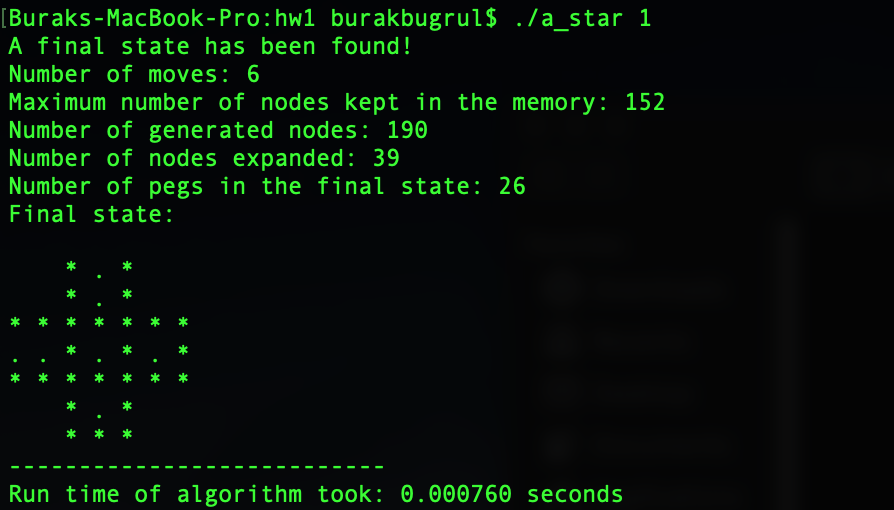
\includegraphics[width=\linewidth]{images/a_star_1.png}
			\caption{A* with Hole Heuristic.}
		\end{subfigure}
		\begin{subfigure}[b]{0.42\linewidth}
			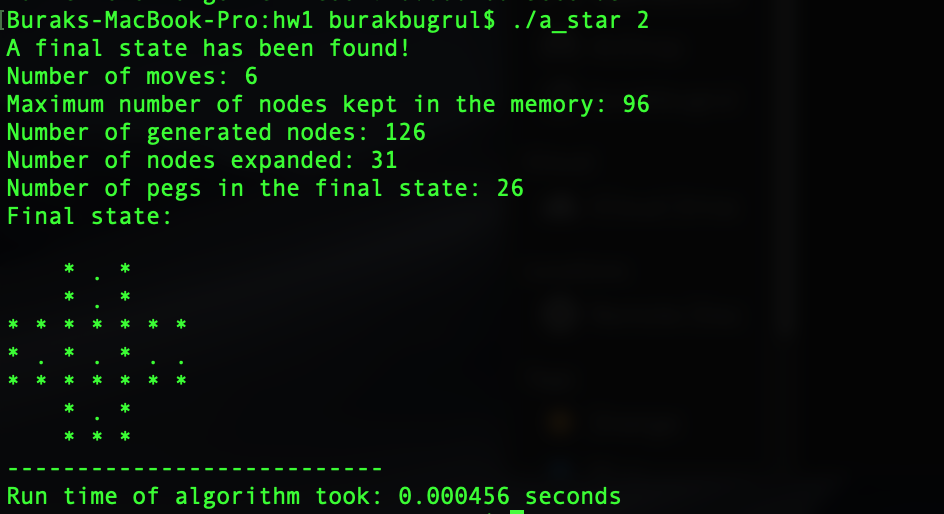
\includegraphics[width=\linewidth]{images/a_star_2.png}
			\caption{A* with Peg Heuristic}
		\end{subfigure}
		\caption{A*}
		\label{fig:A*}
	\end{figure}

	\part{One Peg State} \\ \ \\
	
	If objective was trying to reach a state that has one peg there will be no optimal solution because every action removes exactly one peg. Every valid solution will have 31 actions because there are 32 pegs in the beginning. In this problem BFS will expand all search space whic is not optimal in terms of memory. DFS will use memory more efficiently but it can try very wrong(not necessary) actions in the deeper states. A* with a good heuristic can find a valid final state in a short time.

\end{document}